%%%%%%%%%%%%%%%%%%%%%%%%%%%%%%%%%%%%%%%%%%%%%%%%%%%%%%%%%%%%%%%
%
% Welcome to Overleaf --- just edit your LaTeX on the left,
% and we'll compile it for you on the right. If you open the
% 'Share' menu, you can invite other users to edit at the same
% time. See www.overleaf.com/learn for more info. Enjoy!
%
%%%%%%%%%%%%%%%%%%%%%%%%%%%%%%%%%%%%%%%%%%%%%%%%%%%%%%%%%%%%%%%
\documentclass[border=10pt]{standalone}
%%%<
\usepackage{verbatim}
%%%>
\usepackage{pgfplots}
\pgfplotsset{width=7cm,compat=1.8}
\begin{comment}
:Title: Bar plot
:Tags: 2D;Bar plots;Manual
:Author: Christian Feuersänger
:Slug: bar-plot

Bar plots place horizontal or vertical bars at coordinates. Multiple bar plots
in one axis can be stacked on top of each other or aligned next to each other.

The code is from the PGFPlots 1.10 manual: "4.5.4 Bar Plots".
\end{comment}
\begin{document}
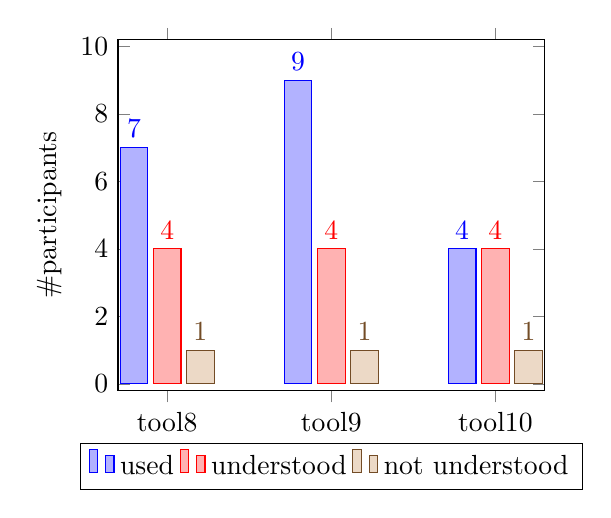
\begin{tikzpicture}
\begin{axis}[
    ybar,
    enlargelimits=0.15,
    legend style={at={(0.5,-0.15)},
      anchor=north,legend columns=-1},
    ylabel={\#participants},
    symbolic x coords={tool8,tool9,tool10},
    xtick=data,
    nodes near coords,
    nodes near coords align={vertical},
    ]
\addplot coordinates {(tool8,7) (tool9,9) (tool10,4)};
\addplot coordinates {(tool8,4) (tool9,4) (tool10,4)};
\addplot coordinates {(tool8,1) (tool9,1) (tool10,1)};
\legend{used,understood,not understood}
\end{axis}
\end{tikzpicture}
\end{document}